%The computational model of Lazy Shadowing has been continuously optimized to improve its scalability and efficiency, to eliminate vulnerability, and to reduce implementation complexity and overhead. This section presents the system design of Rejuvenating Shadows. 

%\subsection{Fault model}

We adopt the fail-stop fault model, which defines that a process halts in response to a failure and its internal state and memory contents are irretrievably 
lost~\cite{Schlichting1983}. Furthermore, we assume that the machine on which failure occurred can be rebooted (or equally, a spare machine is available) for starting a new process after the failure. Note that this is the same assumption for checkpointing/restart. Below we discuss the components of the Rejuvenating Shadows model and its design trade-offs.
 
%As demonstrated in~\cite{cui_2016_scalcom}, Lazy Shadowing is able to tolerate both hardware and software failures under the fail-stop fault model. In this work, we continue with the assumption of fail-stop model. In order to further improve resilience and efficiency, however, Rejuvenating Shadows differentiates between temporary failures and permanent failures. Temporary failures include memory bit flips, kernel panic, etc., and can be recoverd by rebooting the machine, while permanent failures, such as failure in power supply and network switch, needs the device to be replaced in order to recover. Rejuvenating Shadows maximizes the resource utilization for resilience by adopting different strategies for different types of failures. 

\subsection{Shadowing}
\label{sec:shadow}
Shadowing is the essential concept that associates each original process (referred to as main) with a replica process (referred to as shadow), which potentially lower its execution rate to save power. Then fault tolerance comes from the property that if one process fails, its associated process can continue to complete the task. For example, if a main fails, its shadow will be promoted to a new main and continue to carry out the task. 
%In this way, shadow processes are substitutes for mains in the case of failure. 
In this work, however, we deviate from the original concept of shadow as a replica~\cite{cui_2016_scalcom}, and use a shadow as a ``rescuer" to a main in the presence of failures. Specifically, if a main fails, a new main process will be rejuvenated from its associated shadow with our leaping technique, while the shadow remains as a shadow. 

%\subsection{Consistency}
%\label{sec:consistency}

State consistency between mains and shadows is required both during normal execution and following a failure. % of a main process to roll-forward the shadows. 
We designed a protocol, as shown in Figure~\ref{fig:cons_protocol}, 
to enforce sequential consistency, i.e., each shadow sees the same message order and operation results as its main. 
%In this figure, A and B represent two mains, and A' and B' are their shadows. 
For each message, the main of the sender sends a copy of the message to each of the main and shadow of the receiver, and the shadow of the sender is suppressed from sending out messages. We assume that two copies of the same message are sent in an atomic manner, as this multicast functionality 
can be implemented within NIC. The SYNC message in Figure~\ref{fig:cons_protocol} is only used when there is potential non-determinism. This will be discussed in details in the next Section.


\begin{figure}[!t]
  \begin{center}
      	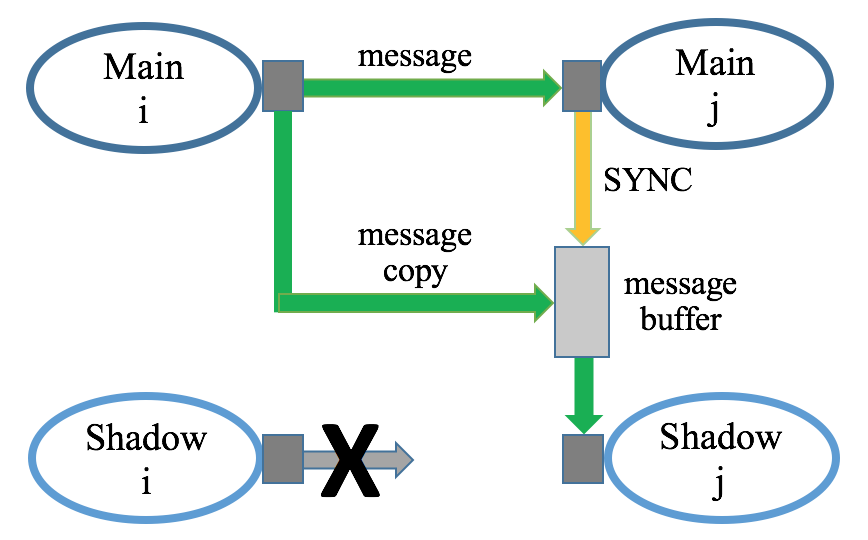
\includegraphics[width=0.7\columnwidth]{figures/consistency}
  \end{center}
  %\vskip -0.25in
  \caption{Consistency protocol for Rejuvenating Shadows.}
  \label{fig:cons_protocol}
\end{figure}

%The SYNC message in Figure~\ref{fig:cons_protocol} is only used when there is potential non-determinism. This will be discussed in details in the next Secton.
%We assume that only MPI operations can introduce non-determinism. MPI\_ANY\_SOURCE may result in different message receiving orders between a main and its shadow. To deal with this, we serialize MPI\_ANY\_SOURCE message receiving by having the main first do the receiving and then use a SYNC message to forward the message source information to its shadow, which then issues a receiving with the specific source. Other operations, such as MPI\_Wtime() and MPI\_Probe(), can be dealt with in a similar manner by forwarding the result from a main to its shadow.

\subsection{Leaping}

Leaping is initially proposed as a technique to boost performance in \cite{cui_2016_scalcom}. As the shadows execute slower than mains, failure recovery introduces delay to the execution. Leaping opportunistically takes advantage of the recovery time and transfers state from each living main to its associated shadow. As a result, shadows achieve forward progress with minimal overhead, and recovery time for future failures, if any, is minimized. 

Recently, we realized that leaping can also be used for rejuvenation (discussed below) to transfer state from a living shadow to a newly started main. Note that leaping always happens between a pair of main and shadow. To avoid ambiguity, the process which provides state in a leaping is referred to as target process, and the other process which receives and updates state is referred to as lagging process. 

%Recently, we have identified an empirical problem to which leaping is a solution. When Lazy Shadowing is used to execute an MPI application, application messages are generated at the rate of the mains, but consumed by the shadows at a lower rate because the shadows are slower. As a result, messages accumulate on the shadow side and could possibly result in a buffer overflow. Leaping is naturally a solution to this problem as it can move the shadows forward and synchronize their execution states with those of the mains. After the synchronization, accumulated messages at the shadows become obsolete and thus can be safely discarded. To differentiate the two cases where leaping is used, leaping during failure recovery is referred to as failure induced leaping while leaping to avoid buffer overflow is referred to as forced leaping. 

\subsection{Rejuvenation}

It has been discussed in ~\cite{cui_2016_scalcom} that each shadowed set can only tolerate one failure. After the first failure, all main processes in the shadowed set would lose their shadows and become vulnerable. Although quantitative study show that a second failure in a shadowed set is unlikely, % even with over one million processes, 
in practice the system will become more and more vulnerable as failures occur. In many cases, it is too costly to take such risk, especially for long-running, large-scale, and mission-critical applications. Therefore, it is preferable to maintain the same level of resilience at all times.

Not surprisingly, vulnerability could be avoided by rejuvenation, in which we restart a new process for every failed process (either main or shadow). In this way, every main is always guaranteed to have an associated shadow, and shadow never needs to substitute a main. The problem, however, is that the newly launched process will start from the beginning and may lag far behind the other processes. Later on when the new process needs to participate in a synchronization point, or when it needs to carry out a failure recovery, significant delay will incur as a result of its lag. 

Fortunately, leaping is a natural solution. After a new process is started, we can use leaping to synchronize the new process' state with its associated living process. Hence, lag of the new process is resolved at the minimal cost of a leaping. %Consider a pair of main process, $M$, and shadow process, $S$, for example. If $M$ fails, a new main process will be started to replace $M$, and then a leaping from $S$ will advance the new process to the state of $S$. This is illustrated in Figure~\ref{fig:faulty}. 
Suppose a main $M_i$ fails at $T_0$, Figure~\ref{fig:rejuvenation} illustrates the failure recovery process with rejuvenation. 
In order for its shadow $S_i$ to speed up and finish the recovery as soon as possible, 
we will temporarily suspend the execution of the other shadows that collocate with $S_i$. %, so that $S_i$ can increase its execution rate and finish the recovery as soon as possible. 
Meanwhile, the failed machine is rebooted and then used to launch a new process for $M_i$. When $S_i$ catches up with the state of the previous $M_i$ before the failure at $T_1$, leaping can be used to advance the new $M_i$ to the current state of $S_i$. The leaping is initiated after $S_i$ catches up so as to avoid the need of message logging for restarting $M_i$. Because of the failure of $M_i$, the other mains will be blocked when they arrive at the next synchronization point, which is also assumed at $T_0$. During the idle time, we can opportunistically perform a leaping and transfer state from each living main to its associated shadow. Therefore, this leaping has minimal overhead as it overlaps with the recovery, as shown in Figure~\ref{fig:non_faulty_diff}. Leaping for the shadows collocated with $S_i$ are delayed until the recovery completes at $T_1$, since these shadows are suspended during the recovery. After the leaping finishes at $T_2$, all mains and shadow can resume normal execution with the same level of resilience as before the failure.

Figure~\ref{fig:rejuvenation} and the above analysis assume that the time for rebooting is no longer than the recovery time. If the new $M_i$ is not yet ready when $S_i$ catches up at $T_1$, however, we have two design choices: 1) $S_i$ can continue execution and take the role of a main; or 2) $S_i$ can wait for the rebooting to finish and the new $M_i$ to launch, and then perform the leaping.  The first option requires a shadow to starting sending out messages, as well as all the other processes to update their internal process mapping in order to correctly receive messages from this shadow (see Figure~\ref{fig:cons_protocol}). This not only complicates the implementation, but also requires expensive global coordination that is detrimental to scalability. We therefore chose the second design.


%On the other hand, if $S$ fails, a new shadow process will be started and immediately advanced to the state of $M$ by leaping.

\begin{figure}[!t]
	\begin{center}
		\subfigure[Faulty task]
		{
			\label{fig:faulty}
			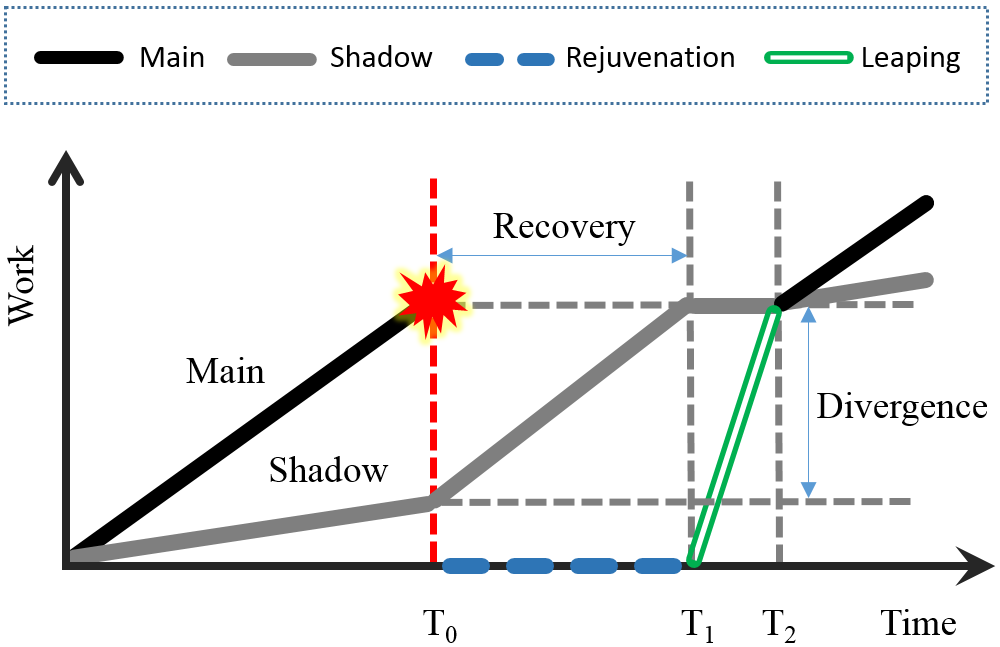
\includegraphics[width=0.7\columnwidth]{figures/rs1}
		}
		\subfigure[Non-faulty tasks in different shadowed sets]
		{
			\label{fig:non_faulty_diff}
			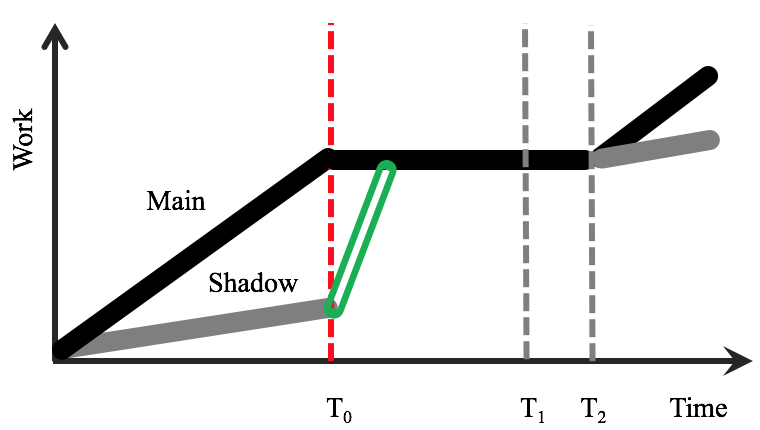
\includegraphics[width=0.7\columnwidth]{figures/rs2}
		}
		\subfigure[Non-faulty tasks in the same shadowed set]
		{
			\label{fig:non_faulty_same}
			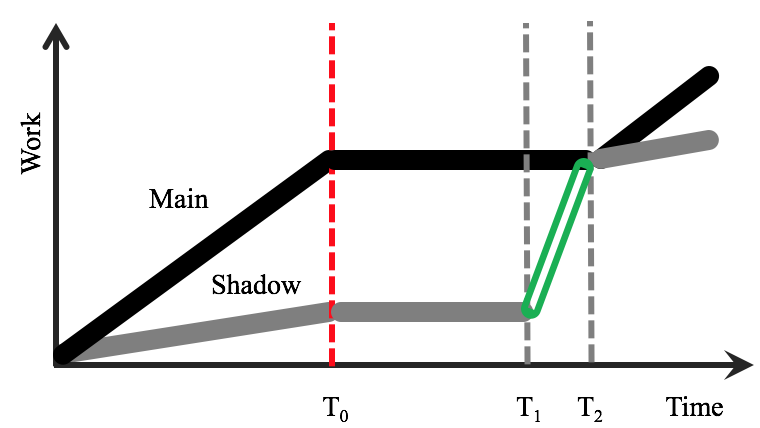
\includegraphics[width=0.7\columnwidth]{figures/rs3}
		}
	\end{center}
	\caption{Recovery and rejuvenation after a main process fails.}
	\label{fig:rejuvenation}
\end{figure}

%Depending on the type of failure, the new process will be placed at different locations. If it is a temporary failure, the node where failure occurs will be rebooted and then used to host the new process, whether it is a main or shadow. Although there is a delay from the rebooting, it is usually small compared to application's running time and can be accounted part of the recovery. 
%For permanent failures, the node cannot be used and we have to migrate and collocate some processes. If the new process is a main, its existing shadow will be migrated to another node where shadow process(es) reside, and make room for the new main. Otherwise, if the new process is a shadow, it will be directely created on a shadow node. 